\documentclass[UTF8]{article}
\usepackage{CTEX}
\usepackage{amsmath}
\usepackage{subcaption}
\usepackage{graphicx}
\usepackage{siunitx}
\usepackage{booktabs}
\usepackage{float}
\usepackage{amssymb}

\begin{document}
    \section{研究背景与问题重述}
    \subsection{研究背景}
    随着经济的快速发展,城市机动车保有量持续上升,居民出行机不可挡。随着交通运输水平的提高,对交通运输的总需求不断增加。如今,主要城市道路日益拥挤被认为是世界上普遍的现象一个社会问题,
    它的出现使得城市的可持续发展轨迹与人民的日常生活和工作秩序发生了严重的质的变化。
    道路基础设施增长速度远不如机动车的增长速度快需求与交通供给不平衡,导致交通频繁拥堵,给城市交通形势带来了新的挑战[2]。为了缓解交通拥堵造成的经济负增长和人们生活工作秩序的混乱,
    对交通状态进行评价是非常必要的。对于城市交通管理者来说,如何快速准确地发现交通拥堵,并根据拥堵程度采取有效的对策,对于缓解交通拥堵有着重要的作用。
    交通参与者可以根据交通状态信息选择更平坦的道路线路出行可以缓解路段拥挤的压力,达到减少交通拥堵的程度。\\
    道路交叉口是车辆和行人聚集、转弯和疏散的场所,是交通的咽喉。因此,正确设计交叉口道路,合理组织、管理交叉口交通,是提高道路通行能力和保证交通安全的重要手段。
    从交通拥堵评价的相关研究来看,现有的评价方法主要集中在道路和路网的评价上,相关的评价指标主要包括交叉路口饱和度、平均停车延误、交叉口速度比、交通密度等状态指标[3]。
    由于数据采集手段的限制,无法准确采集评价模型中的一些参数。虽然一些新的探测设备已经投入市场,但由于建设成本和探测效果的影响,国内城市还没有大规模安装。\\
    \subsection{问题重述}
    以上述背景为契机,题目提供了多功能电警数据(流量和车尾时距)。为了建立一个路口交通状态的评价模型,在题目已给的数据上进行数学建模,且需要回答以下两个问题:\\
    (1)基于所提供的数据,和现有的评价指标建立一个能够评价路口交通状态的数学模型。\\
    (2)基于所提供的数据和第一问的模型,建立数学模型用于路口信号灯配时方案的调优工作。
    \section{模型假设与符号说明}
    \subsection{模型假设}
    (1)假设汽车在经过交叉路口后分别在四条道路的区间速度是均匀的;\\
    (2)假设汽车在观山东路和长岭路交叉路口通过红绿灯的速度为最大限速30码;\\
    \subsection{符号说明}
    
    \begin{table}[H] 
        \centering
        \caption{符号说明}
         \tiny
         \label{table_time}
         \resizebox{\textwidth}{!}{
         \begin{tabular}{lllllll}
         
        \toprule  
         
          指标符号 & 符号说明  & 单位 \\
               
         
        \midrule  
         
          $\mathcal{Q}$  & 某一方向的车流驶入量 & ——  \\ 
         
          $\tilde{v}$  & 平均车尾时距 &   $s$  \\
          $v_i(i=1,2,3,4)$ & 东南西北四个方向平均速度 & $m/s$\\
          \bottomrule 
         
        \end{tabular}
         }
        \end{table}
    \section{数据预处理}
    \subsection{交叉运行状态评价指标}
    根据城市道路交叉口的功能及交通特性,本文使用的交叉口评价指标包括:交通量、平均速度比、平均车尾时距。
    \subsubsection{交通量}
    交通量是指单位时间内通过道路某断面的交通流量(即单位时间通过道路某断面的车辆数目)。\\
    本文数据为3月2号到3月8号贵阳长岭路与观山东路车尾一周的时序数据,根据每抓怕一次就代表有一辆车经过的原则,可以计算出每天各路口各车道的车量总数,即日交通流,见附件。\\
    
    \begin{table}[H]
        \centering
        \caption{3月2号到3月8号各转向的车流量}
        \begin{tabular}{cccccccc}
           \hline
            转向/日期 & 2号 & 3号 & 4号 & 5号 & 6号 & 7号 & 8号 \\
           \hline
            东向西左转1	& 2935	&2942	&2949	&3091	&3003	&2289	&3168\\
           
            向西左转+直行2	&2864 &2870	&2984	&2671	&2632	&2276	&2733\\
           
            东向西直行3	&7333	&7247	&7541	&7112	&4333	&1833	&2268\\
           
            东向西直行4	&6389	&6509	&6555	&6217	&3574	&1569	&2068\\
           
            东向西右转5	&5286	&5349	&5637	&5168	&3458	&1510	&1798\\
           
            西向东左转1	&1886	&2171	&2553	&2350	&2153	&1802	&2595\\
           
            西向东左转2	&1971	&2103	&2210	&2066	&2103	&1592	&2355\\
           
            西向东左转3	&4316	&4488	&4822	&4627	&4682	&3687	&4369\\
           
            西向东直行4	&6569	&6013	&5852	&5453	&5205	&4307	&5382\\
           
            西向东东直行5	&6880	&6671	&7767	&7278	&6863	&6112	&4760\\
           
            西向东直行6	&4974	&4752	&5414	&5083	&4629	&3885	&3051\\
           
            西向东右转+直行7	&3921	&3587	&4360	&3529	&3274	&2951	&2383\\
           
            南向北左转1	&2022	&1979	&2030	&1668	&1445	&1648	&1911\\
           
            南向北左转2	&2319	&2234	&2249	&2014	&1764	&1894	&2120\\
           
            南向北左转3	&2184	&2196	&2358	&1940	&1749	&1785	&1911\\
           
            南向北直行4	&2187	&2396	&3235	&3045	&2878	&2316	&3080\\
           
            南向北直行5	&2186	&2496	&3117	&3034	&2770	&2340	&3196\\
           
            南向北直行6	&1995	&2323	&2752	&2711	&2361	&1929	&2931\\
           
            南向北直行7	&1791	&2065	&2487	&2294	&1895	&1533	&2598\\
           
            南向北右转+直行8	&1218	&1415	&1790	&1550	&1308	&1176	&1770\\
                       
            南向北右转9	&5323	&5739	&7417	&6565	&5893	&4569	&6752\\
           
            北向南左转1	&1517	&1530	&1469	&1344	&1254	&1193	&1335\\
           
            北向南左转2	&1860	&1887	&1793	&1786	&1619	&1523	&1635\\
           
            北向南左转3	&1989	&2065	&1871	&1873	&1723	&1582	&1785\\
           
            北向南左转+直行4	&6165	&6095	&6349	&5814	&5769	&5122	&6931\\
           
            北向南直行5	&7357	&7589	&7591	&7193	&7058	&6363	&8627\\
           
            北向南直行6	&7018	&7102	&7177	&6269	&6242	&5586	&7524\\
           
            北向南直行7	&899	&961	&814	&769	&684	&631	&785\\
           
            北向南右转+直行8	&1155	&1228	&1036	&1035	&873	&804	&995\\
           
            北向南右转9	&1132	&1296	&1044	&1104	&994	&833	&1045\\
           
            总计	&105641	&107298	&115223	&106653	&94188	&76640	&93861\\
           \hline
            
        \end{tabular}
    \end{table}
    由表 1可知3月4号,即星期五的车流量最高,且北向南左转+直行4、北向南直行5、
    北向南直行6、南向北右转9、东向西直行3等路线的日交通流相对较大。分别达到了6349、7591、7177、7417、7541车次。\\
    以30分钟为一个时间段,上北下南,左西右东为方向,将30个转向划分为向北驶入车辆、向西驶入车辆、向南驶入车辆、向东驶入驶入,则可以统计出7天内共336个时间段向北、向西、向南、向东这四个方向的汽车驶入量,记为$Q_ij$  ,其中$i=1,2,3,4$,代表向北、向西、向南、向东驶入,$j=1,⋯,336$,代表第$j$个时间段。各方向划分,见图 1\\
    \begin{figure}[H]
        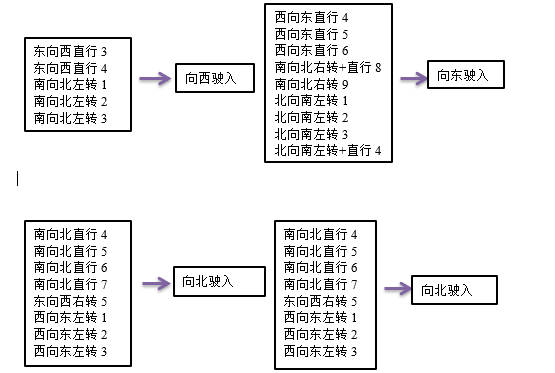
\includegraphics[width=\linewidth]{1.jpg}
        \caption{划分准则}
        \label{fig:ph1}
    \end{figure}
    \subsubsection{车尾时距}
        忽略车的长度,将当次抓拍时间与上一次抓拍相减得到的时间差等价于这两辆车的时间距。\\
    根据上一节的划分,可以得到在各时间段内向北、向西、向南、向东驶入的数据,再计算出各时间段内向北、向西、向南、向东驶入的时间距总和,记为$T_ij$  ,其中$i=1,2,3,4$,代表向北、向西、向南、向东驶入,j=1,2,...,336,代表第j个时段。根据公式(1)可得第j个时间段向i驶入的平均时间车尾时距$V ̃_ij$\\
    \begin{equation}
        V ̃_ij=\frac{Q_{ij}}{T_{ij}} \quad i=1,2,3,4; j=1,2,⋯,336	
    \end{equation}
        
    \subsubsection{平均速度}
    查阅网上资料,知道长岭路与观山东路交叉路口到林城东路与长岭北路交叉路口、山东路环形桥、长岭南路、观山东路的长度$S_1、S_2、S_3、S_4$,时间分别为:$T_1、T_2、T_3、T_4$,且到该区段红绿灯的限速度为30码,换算后$ v ̂=8.3m/s$根据公式(1)可得该交叉路口四个方向的区间平均速度$v_i$。
        \begin{equation}
            v_i=\frac{S_i}{T_i}     \quad           i=1,2,3,4	
        \end{equation}	
        根据以上陈述可得图 2\\
    \begin{figure}[H]
        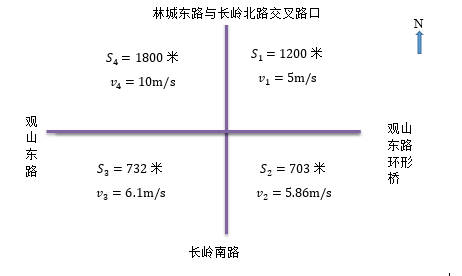
\includegraphics[width= \linewidth]{2.jpg}
        \caption{区平均速度}
    \end{figure}
    将数据整理,可得到一个$1344×5$的数据表,其中列名分别为车辆驶入方向、时间、流量、车尾时距、平均速度,数据如表3\\
    \begin{table}[H]
        \centering
        \caption{数据表}
        \begin{tabular}{ccccc}
            \hline
            时间 & 方向 & 流量  & 车尾时距 & 平均速度(m/s)\\
            \hline
            00:00:00-00:30:00	&EAST	&419	&41.9642	&5.86\\
            00:00:00-00:30:00	&SOUTH	&159	&44.7862	&6.1\\
            00:00:00-00:30:00	&WEST	&73	&131.7808	&10\\
            00:00:00-00:30:00	&NORTH	&213	&61.9859	&5\\
            00:30:00-01:00:00	&EAST	&340	&52.8706	&5.86\\
            00:30:00-01:00:00	&SOUTH	&154	&56.70778	&6.1\\
            00:30:00-01:00:00	&WEST	&44	&202.2045	&10\\
            00:30:00-01:00:00	&NORTH	&146	&101.7260	&5\\
            …	&…	&…	&…	&…\\
            23:30:00-00:00:00	&EAST	&0	&0	&5.86\\
            23:30:00-00:00:00	&SOUTH	&0	&0	&6.1\\
            23:30:00-00:00:00	&WEST	&1010	&50.3623	&10\\
            23:30:00-00:00:00	&NORTH	&0	&0	&5\\
            \hline
        \end{tabular}
    \end{table}
    \section{模型建立与求解}
    \subsection{问题一}
    \subsubsection{问题一的分析}
     问题一要求我们使用附件中的数据,建立一个能够评价路口交通状态的数学模型。依据现有的评价指标,流量、交叉路口平均速度比和车尾时距,使用灰色关联分析、聚类分析和秩和比综合评价法建立城市交通状态评价体系,问题一的思维结构图如图3所示。\\
     \begin{figure}[H]
         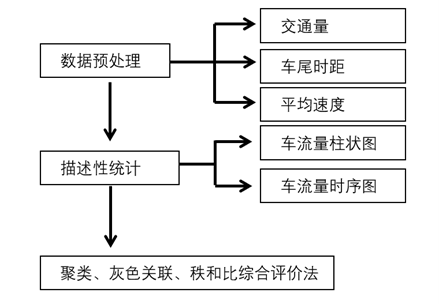
\includegraphics[width=\linewidth]{2.png}
         \caption{问题一处理流程图}
     \end{figure}
     \subsubsection{模型介绍}
     \textbf{(1)描述性统计分析}\\
        描述性统计是指使用表格和分类、图形和一般数据计算来描述数据特征的各种活动。描述性统计分析统计描述调查中所有变量的相关数据,主要包括数据频率分析、集中趋势分析、离散度分析、分布和一些基本统计图形。\\
        ① 数据的频率分析。在数据预处理部分,可以通过频率分析和交叉频率分析来检测异常值。\\
        ② 数据的集中趋势分析。它用于反映数据的总体水平。常用的指标包括平均值、均值。\\
        ③ 绘制统计图表。用图形表示数据比用文字表示数据更清晰、更简洁\\
    \textbf{(2)时序图:}\\
         时序图描述对象是如何交互的,并且将重点放在消息序列上。时序图强调消息事件的发生顺序,更方便于阐述事件流的过程。时序图有两个坐标轴:纵坐标轴显示时间,横坐标轴显示对象。步骤为:\\
        ·确定横纵坐标;\\
        ·识别参与过程的交互对象;\\
        ·从初始消息开始,依次画出随后消息。\\
    \textbf{(3)聚类分析}\\
        聚类分析简称为聚类。聚类使得同类中的数据点具有相同的属性或特征
        而类与类的特征明显,常用的类与类的特征有均值(重心)、样本离差阵以及协方差阵与类的直径。聚类又分为样本聚类、变量聚类动态聚类,其中样本聚类又可称系统聚类。常用的聚类方法包括k均值聚类算法(K-Means)、基于密度的聚类算法(DBSCAN)、高斯混合模型(GMM)的最大期望(EM)聚类算法、凝聚层级聚类算法(HAC)、图团体检测聚类算法(GCD)。本文采用K-Means聚类方法,K-Means算法思想较为简单,对于给定的样本集,
        依据样本之间的距离大小,将样本划分为 个簇。使得簇内点紧密相连,
        而簇与簇间距尽可能的大。使用数学表述为:假设将数据划分为$( C_1,C_2,C_3,...,C_k) $,则K-Means的目标为最小化平方误差$E$:
                \begin{equation}
                    E=\sum_{i=1}^k\sum_{x \in C_i}\| x-\mu_i \|_2^2  
                \end{equation}
        其中$\mu_i$是$C_i$的质心,其表达式为:
                \begin{equation}
                    \mu_i = \frac{1}{|C_i|}\sum_{x \in C_i}x 
                \end{equation}
        由此得到传统K-Means算法的一般流程为:\\
            输入样本集$D=\{ x_1,x_2,...,x_n\} $,聚类的簇数为$k$,最大迭代次数为$N$,输出样本集的划分$C=\{ C_1,C_2,C_3,...,C_k\} $。\\
            a.从数据集中随机选择$k$个样本作为质心$\{\mu_1,\mu_2,\mu_3,...,\mu_k \}$。当$n=1,2,3,...,n$时,初始化簇划分为$C_t=\varnothing $,$t=1,2,...,k$。针对每个样本$x_i(i=1,2,3,4,5,...,n)$与质心向量$\mu_j(j=1,2,3,..,k)$计算距离:\\
                \begin{equation}
                    d_{ij} = \|x_i-\mu_j\|_2^2 
                \end{equation}
            并将$x_i$标记为最小$d_{ij}$对应的类别为$\lambda_i$,同时更新$C_{\lambda_i}=C_{\lambda_i}\cup\{x_i\}$。之后对$C_j(j=1,2,3,..,k)$中所有样本点计算质心。当所有$k$个质心都没有发生改变时,输出簇划分$C={C_1,C_2,...,C_k}$。\\
            b. 根据上一步得到到簇划分,求得标签(类别)并绘制聚类结果图。\\
            \textbf{(4)灰色关联分析}\\
            灰色系统理论提出了对各子系统进行灰色关联度分析的概念[5],意图透过一定的方法,去寻求系统中各子系统(或因素)之间的数值关系。因此,灰色关联度分析对于一个系统发展变化态势提供了量化的度量,非常适合动态历程分析。具体步骤如下所示:\\
            ·确定影响特征的参考数列(也称母序列)$Y=Y(k)(k=1,2,..,n)$和比较数列(也称子序列) $X_i=X_i(k)(k=1,2,..,n;i=1,2,...,m)$;
            ·对参考数列和比较数列进行无量纲化处理,主要初值化处理与均值化处理。本文采用初值化处理的方式,具体操作如下:\\
                \begin{equation}
                    x_i(k)=\frac{x_i(k)}{x_i(1)},k=1,2,3,...,n;i=0,1,2,3...,m
                \end{equation}
            其中$k$为时间段,$i$为数列中的一行;\\
            ·求参考数列与比较数列的灰色关联系数,公式如下:\\
                \begin{equation}
                    \zeta_i(k)=\frac{\min\limits_{x}\min\limits_{k}\lvert y(k)-x_i(k)\rvert + \rho\max\limits_{i}\max\limits_{k}\lvert y(k)-x_i(k)\rvert}{\lvert y(k)-x_i(k) \rvert + \rho\max\limits_{i}\max\limits_{k}\lvert y(k)-x_i(k) \rvert} 
                \end{equation}
            记$\Delta_i(k)=\lvert y(k)-x_i(k) \rvert$,则上式可简化为\\
                \begin{equation}
                    \zeta_i(k)=\frac{\min\limits_{i}\min\limits_{k}\delta_i(k)+\rho\max\limits_{i}\max\limits_{k}\delta_i(k)}{\delta_i(k)+\rho\max\limits_{i}\max\limits_{k}\delta_i(k)}
                \end{equation}
            其中$\rho\in(0,\infty)$,称为分辨系数。$\rho$越小,分辨力越大,通常取$\rho=0.5$;\\
            ·计算关联度$\gamma_i$,计算公式如下:\\
                \begin{equation}
                    \gamma_i = \frac{\sum_{k=1}^n \zeta_i}{n},k==1,2,3,...,n;
                \end{equation}
            ·对计算得到的关联度进行排序。\\
            灰色关联度分析对样本量的多少没有过多的要求,对样本不分布规律要求不高,是系统分析中比较简单、可靠的分析方法,对本文的研究对象比较适合。\\
            \textbf{(5)秩和比综合评价法}\\
            秩和比[6][7](RSR)指将效益型指标从小到大排序进行排名、成本型指标从大到小排序进行排名,再计算秩和比,最后统计回归、分档排序。通过秩转换,获得无量纲统计量RSR,以RSR值对评价对象的优劣直接排序或分档排序,从而对评价对象做出综合评价。基本思想是在一个n个评价对象和m个评价指标或等级矩阵中,通过秩转换,获得无量纲的统计量RSR,以RSR值对评价对象的优劣进行排序,进而根据比较组数的多少,进行分档处理或进行RSR平方根反正弦变换值可信区间处理。它是一组全新的统计信息分析方法,是数量方法中一种广谱的方法,针对性强,操作简便,使用效果明显,兼及描述性与推断性。具体步骤如下:\\
            准备好数据,并且进行同趋势化处理与量纲问题;
                ·确认各指标权重;\\
                ·计算秩值,根据每一个具体的评价指标按其指标值的大小进行排序,得到秩次R,用秩次R来代替原来的评价指标值;\\
                ·计算得到RSR值和RSR值排名;
                ·列出RSR的分布表格情况并且得到Probit值;\\
                ·以Probit值(累积频率所对应的概率单位)为自变量,以 RSR 值为因变量,计算直线回归方程,拟合所对应的RSR估计值;\\
                ·根据拟合的RSR值排序,并且进行分档等级。\\
    \subsubsection{描述性统计分析}
        对长岭路和观山东路十字路口3月2号至3月8号东南西北四个方向的车流量进行描述性统计分析,得到东南西北四个路口的频数统计如图:\\
        \begin{figure}[H]
            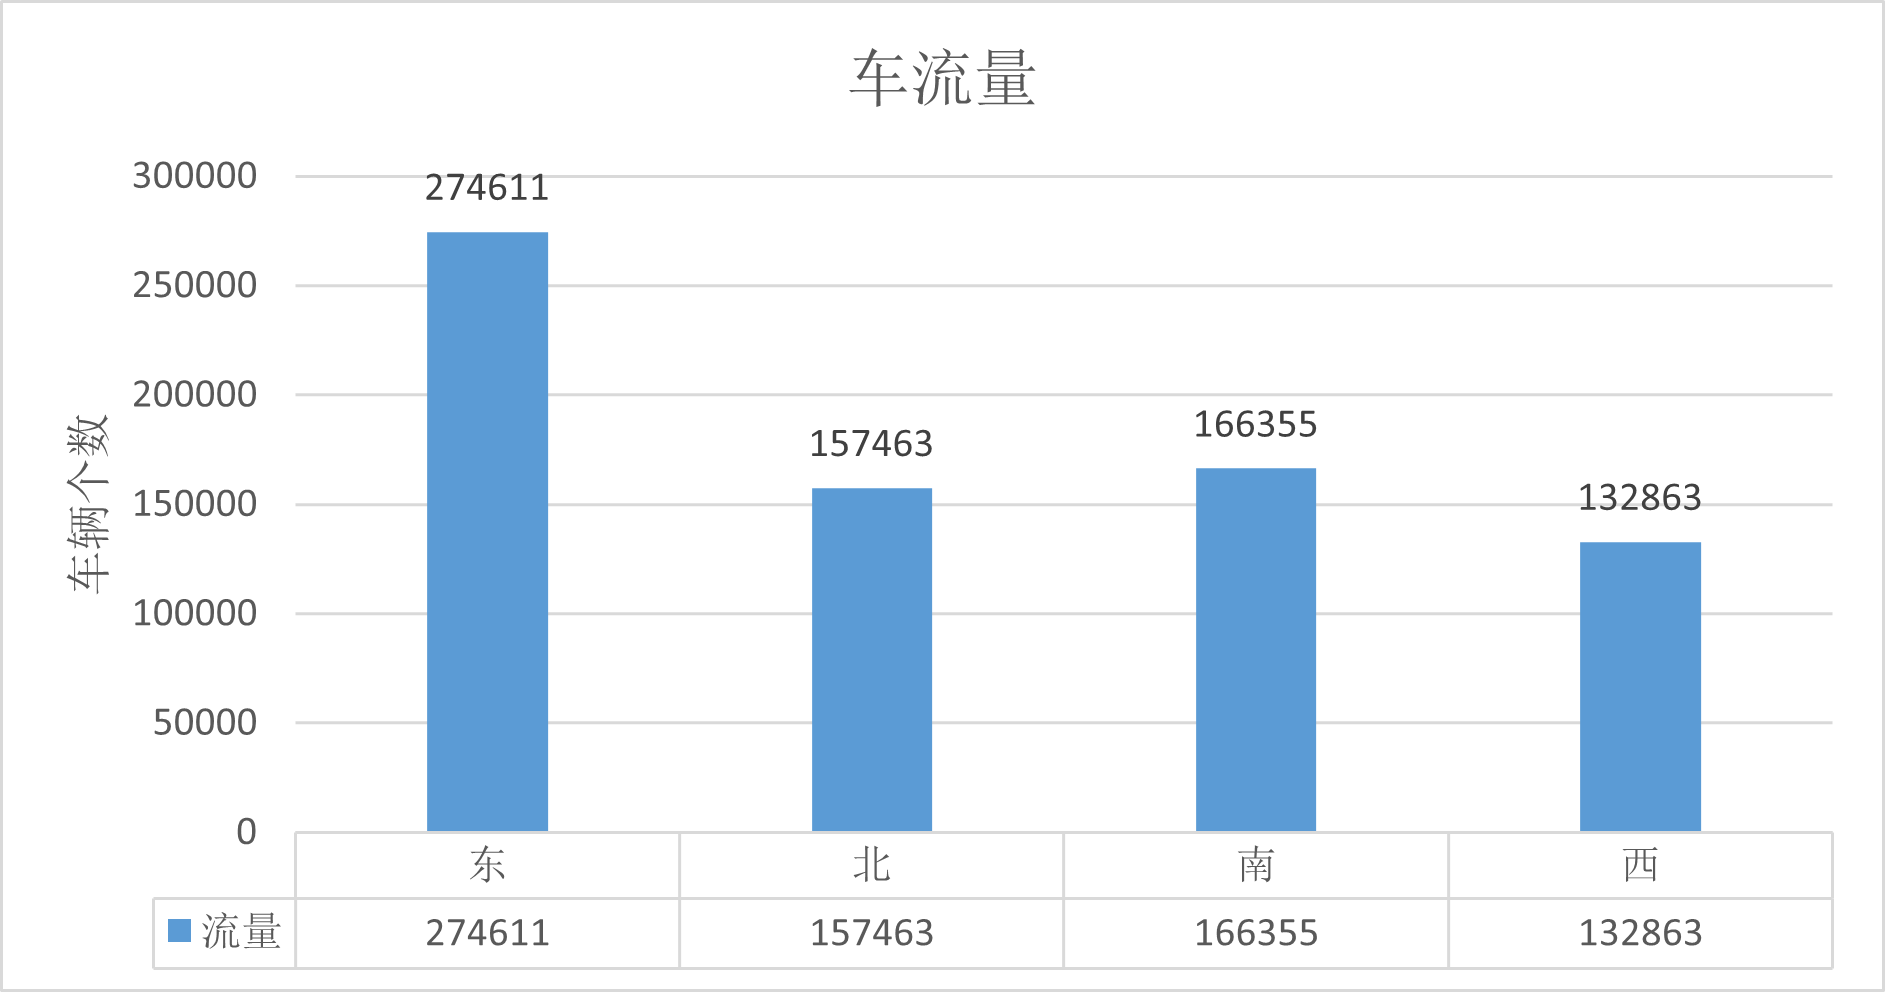
\includegraphics[width=\linewidth]{3.png}\
            \caption{3月2日至3月8日东南西北四方向的车流量}
            \label{fig:f3}
        \end{figure}
        \begin{figure}
            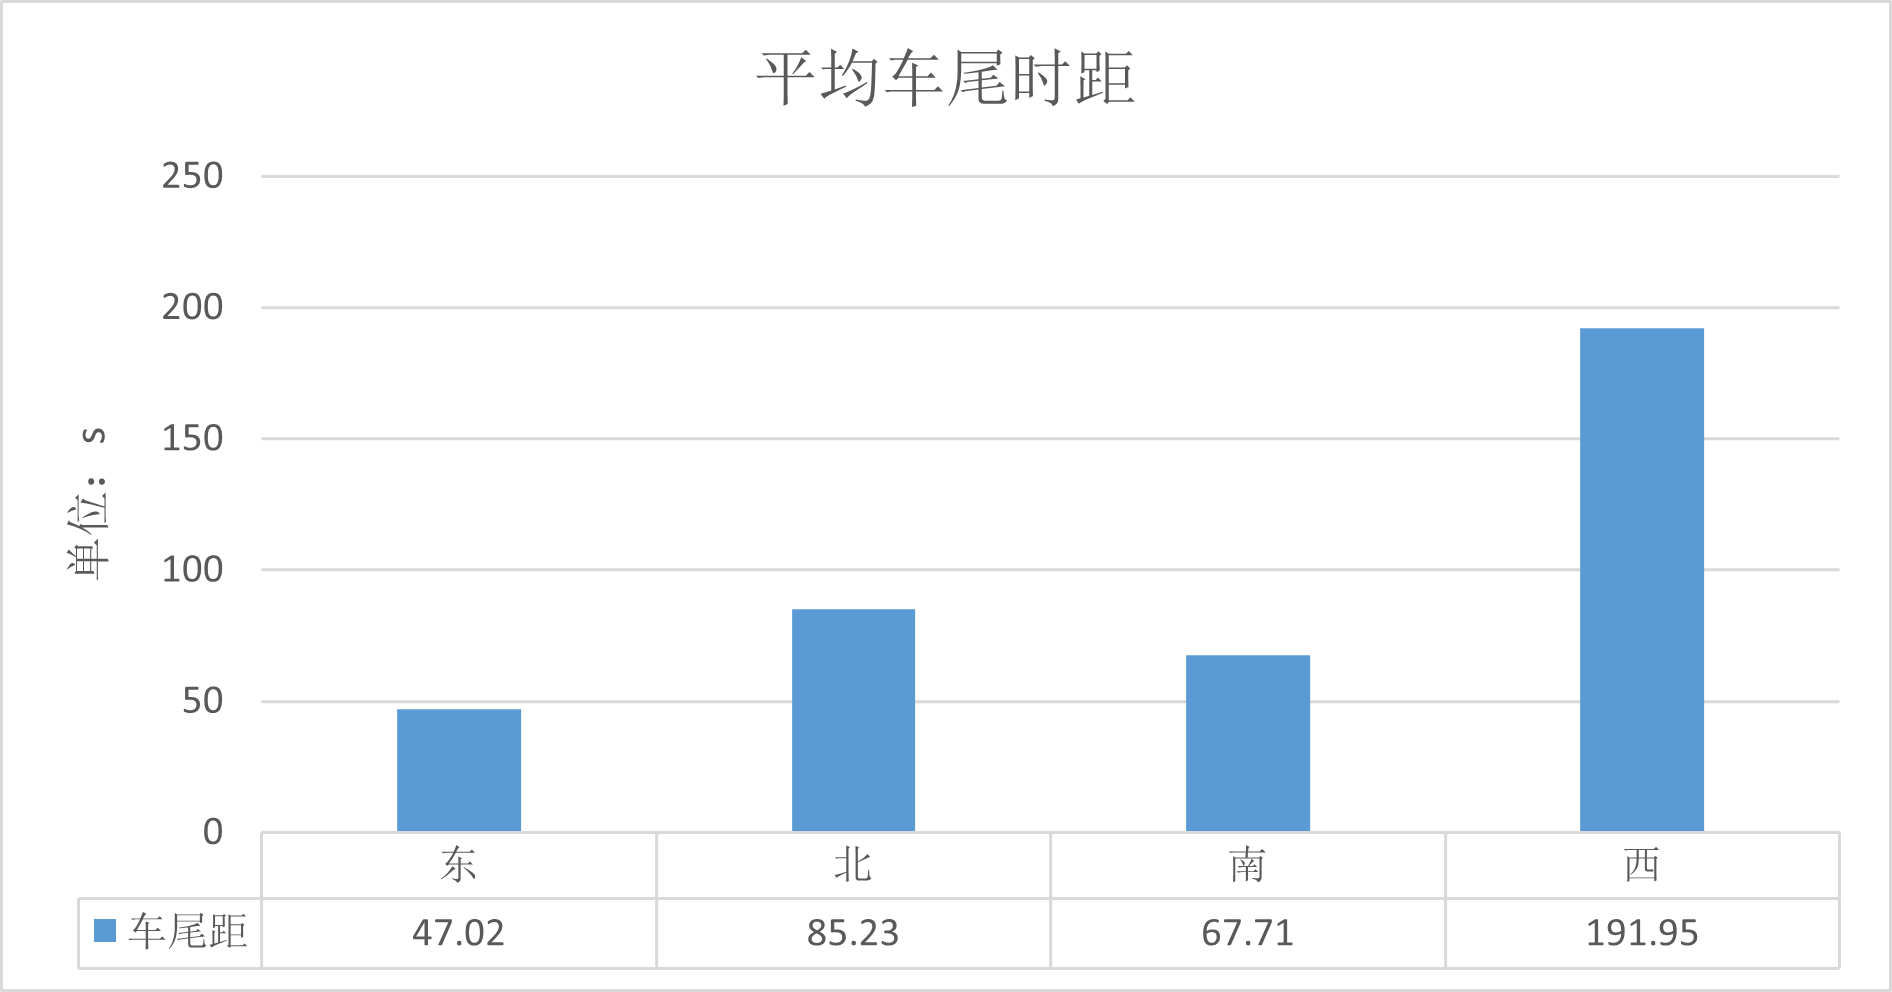
\includegraphics[width=\linewidth]{4.png}
            \caption{3月2日至3月8日东南西北四方形平均车尾时距}
            \label{fig:f4}
        \end{figure}\\
        从图3可以看出在3月2号至3月8号,十字路口向东行驶的车流量最大,达到274611辆,约是向西行驶车辆数的2倍;在这七天中,向西行驶的车流量在这四个方向中比较小。从图4可以看出,由于向东行驶的车流量较大,所以向东行驶的平均车尾时间距里较小,约47s。向西行驶的车流量较少,其平均车尾时间距大。\\
    
    \subsubsection{4.1.4时序图}
    将长岭路和观山东路的十字路口的数据,即表2,画出2号至8号的朝四个方向驶入的流量-时间时序图,如图5、6、7、8、9所示:\\
        \begin{figure}[H]
            \begin{subfigure}[H][0.5\linewidth]
                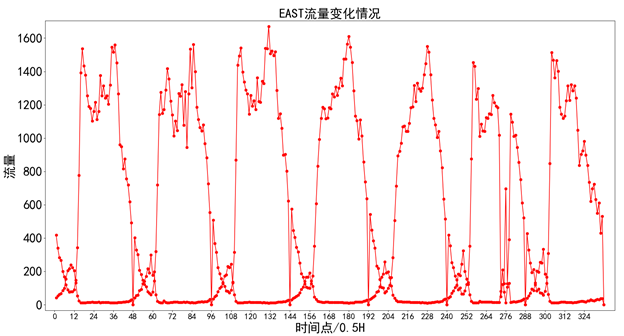
\includegraphics[width=\linewidth]{5.png}
                \caption{2号-8号车流方向为东的流量时序图}
            \end{subfigure}
            \begin{subfigure}[H][0.5\linewidth]
                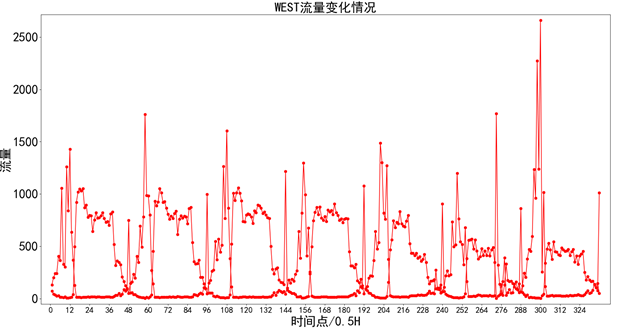
\includegraphics[width=\linewidth]{6.png}
                \caption{2号-8号车流方向为南的流量时序图}
            \end{subfigure}
        \end{figure}
        \begin{figure}[H]
            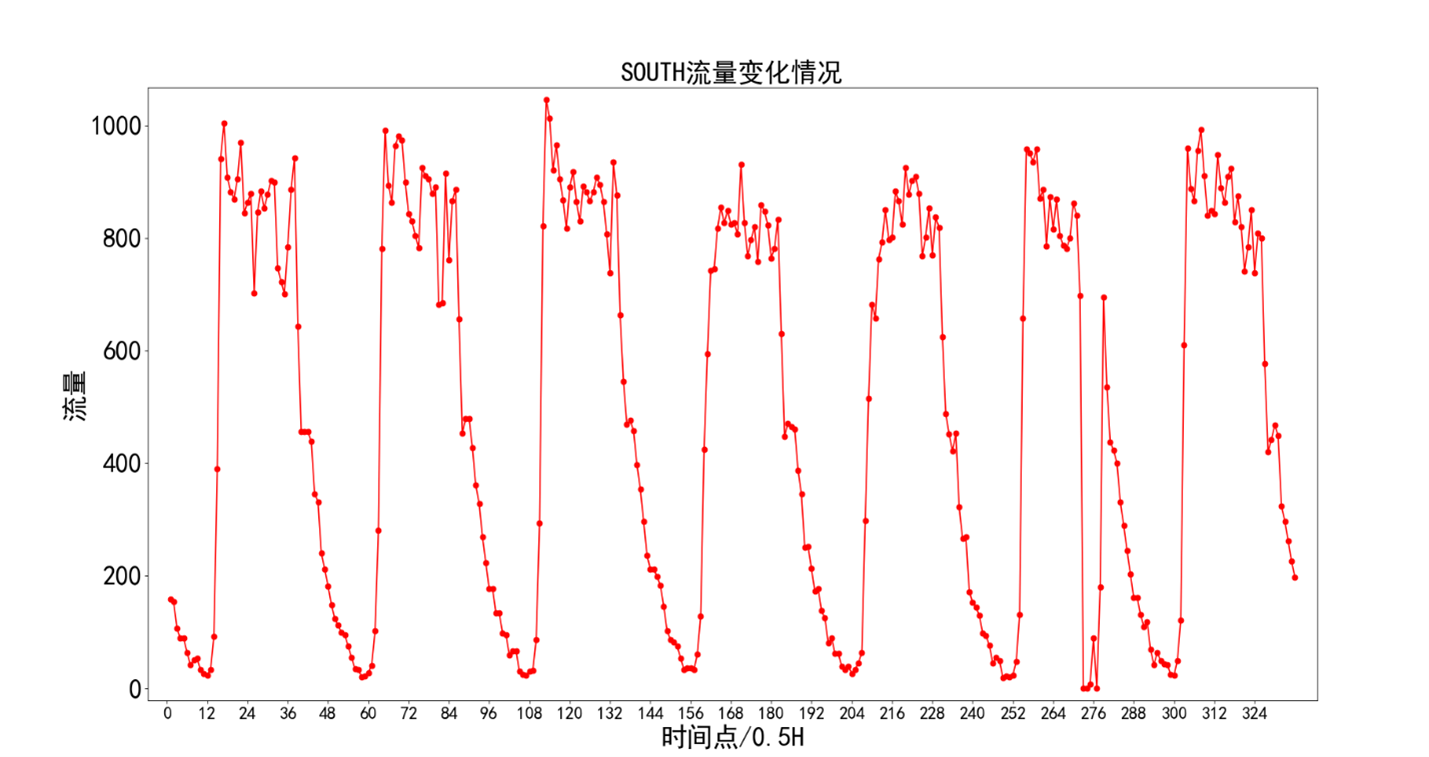
\includegraphics[width=\linewidth]{7.png}
            \caption{2号-8号车流方向为西的流量时序图}
        \end{figure}
        \begin{figure}[H]
            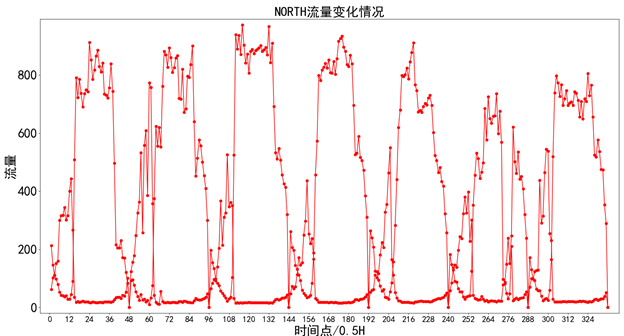
\includegraphics[width=\linewidth]{8.png}
            \caption{2号-8号车流方向为北的流量时序图}
        \end{figure}
        \begin{figure}[H]
            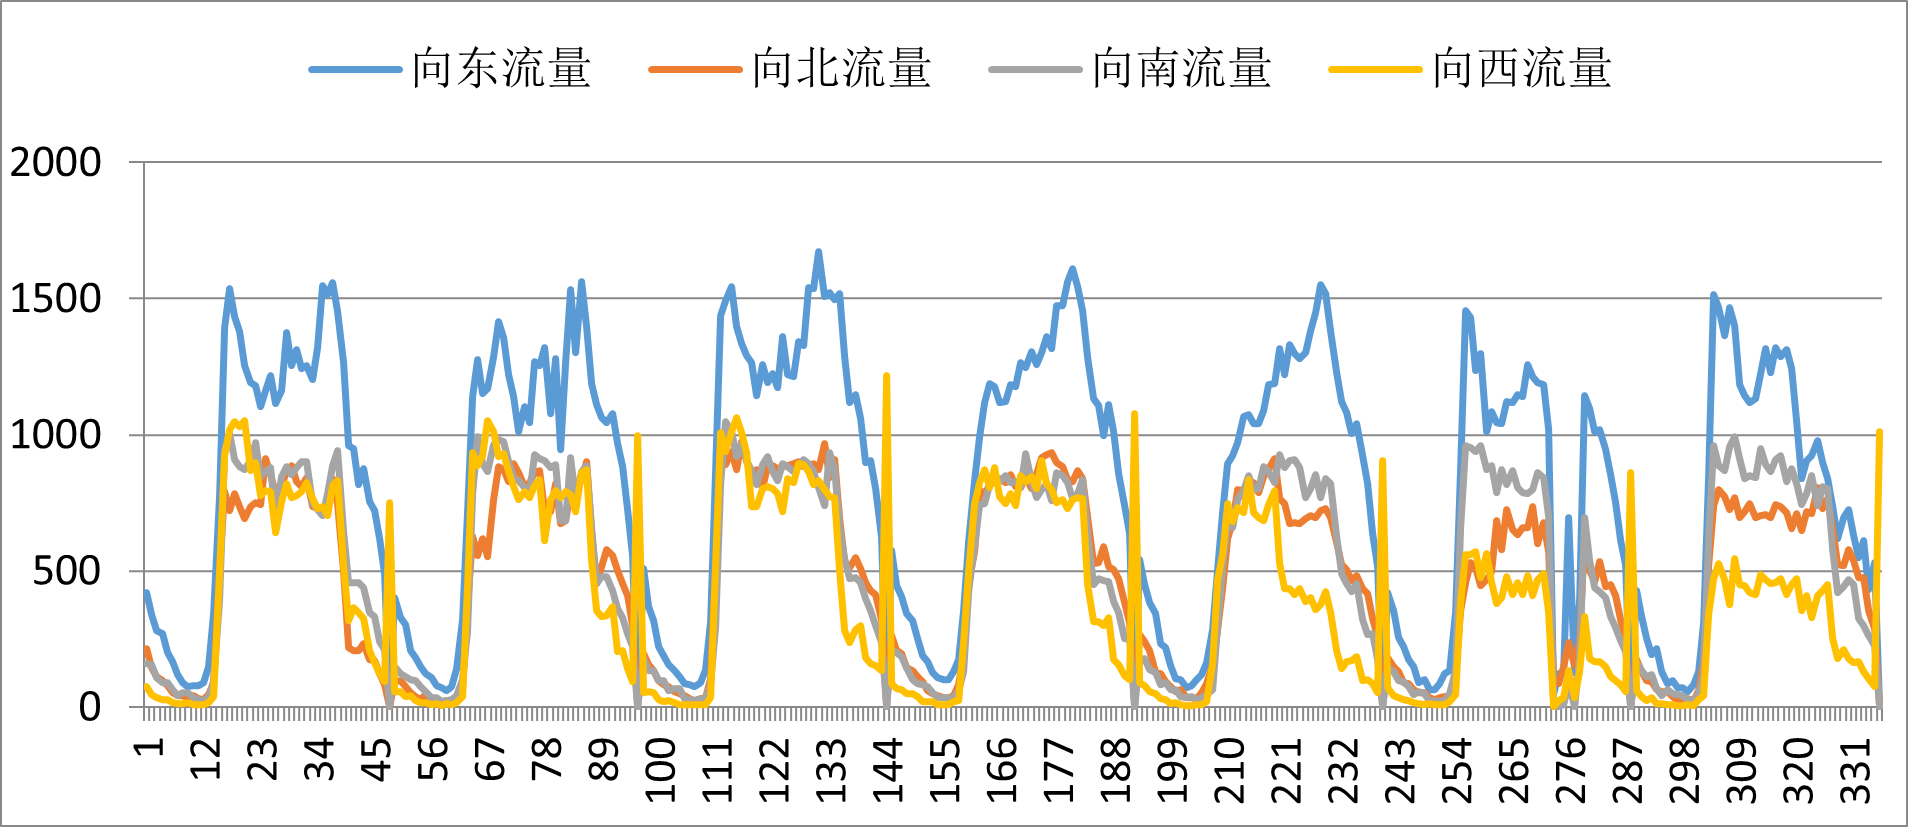
\includegraphics[width=\linewidth]{9.png}
            \caption{2号-8号四方向流量时序图}
        \end{figure}



                
                        



     
            

    


    
\end{document}